\documentclass[11pt, fleqn, a4paper, leqno]{scrartcl} %A4
\usepackage[utf8x]{inputenc} %Eingabe
\usepackage[T1]{fontenc} %Font

\usepackage[ngerman]{babel} %Trennnung
\usepackage{amsmath} %Mathesysmbole
\usepackage{graphicx} %Grafiken
\usepackage{listings} %Programmcode
\usepackage{tikz} %Grafiken malen
\usetikzlibrary{arrows}
\usepackage{hyperref}
\usepackage{dsfont}
\hypersetup{
    colorlinks=true, %set true if you want colored links
    linktoc=all,     %set to all if you want both sections and subsections linked
    linkcolor=blue,  %choose some color if you want links to stand out
}



\title{Zusammenfassung: Modellierung und Simulation}
\author{Andreas Ruscheinski, Christian Delfs}
\date{}
\begin{document}
\maketitle
\tableofcontents
% Verhindert Hurenkinder
\widowpenalty = 10000
% Verhindert Schusterjungen
\clubpenalty = 10000

\section{Hinweis}
Die Urheberrechte der Bilder liegen bei Prof. Adelinde Urmacher, entstammen der Vorlesung "Modellierung und Simulation" aus dem Sommer Semester 2014. Die Texte sind an die Vorlesung angelehnt und entsprechen teilweise dieser. In diesem Fall liegen die Urheberrechte ebenfalls bei Prof. Adelinde Urmacher. Die Autoren übernehmen keine Garantie für Richtigkeit und Vollständigkeit.
\section{Einführung}
	\subsection{Vorbetrachtung}
	\begin{itemize}
		\item Experimente mit dem Computer als Labor
		\item Beispiele: Maschinenanordnung in einer Firma optimieren, Flugzeug fliegen lernen 
		\item Warum: Reale Experimente nicht oder nur teilweise durchführbar (Menschenexperimente, Klimaveränderungen, Entwicklung über mehrere Jahrhunderte)
		\item Risiken: falsche Ergebnisse (Modell passt nicht immer in die Reale Welt, Benutzer obliegt die Verantwortung die Ergebnisse zu interpretieren und kritisch zu hinterfragen)
	\end{itemize}
	\subsection{Definitionen}
	\begin{description}
		\item[System:] Ein System besteht aus Eingaben, Ausgaben und dem Verhalten. Man unterscheidet in Umgebung eines Systems und das Innere eines Systems. Die Umgebung gilt als Abgrenzung. Das Innere beschreibt die Zustände, Komponenten und die Relationen der einzelnen Komponenten. Es muss für jedes System die Systemelemente, Kommunikationsstrukturen und der Veränderung von Werten über die Zeit identifiziert werden.
		\item[Modell:] Ein Modell ist eine Abstraktion eines Systems. Wir stellen ein Modell nur zusammen mit einem System und einem Experiment da. \glqq A model (M) for a system (S) and an experiment (E) is anything to which E can be applied to answer questions about (S).\grqq
		\item[Experiment:] Ein Experiment beinhaltet eine klare Fragestellung (Was soll beantwortet werden?). An ein Experiment sind verschiedene Kriterien gestellt z.b Wiederholbarkeit(unter identischen Voraussetzungen sollen identische Experimente zu den identischen Ergebnissen führen). Wichtig ist dabei die Dokumentation des Experimenten indem die Voraussetzungen, Umgebungsparameter und die Ergebnisse fest gehalten werden. \glqq An experiment is the process of extracting data from a system by excerting it through its input.\grqq
		\item[Simulation:] Eine Simulation ist ein Experiment welches auf einem Modell ausgeführt wird. 
		\item[Computer Modell:] Ein durch einen Computer ausführbares Modell, d.h. definiert in einer durch den Computer interpretierbaren Syntax.
		\item[Computersimulation:] Ein durch einen Computer ausführbares Experiment mit einem computerbasierten Modell.
	\end{description}
\section{Modellierung, Modelle und Sichten}
	\subsection{Wie kommt man von einem System zum Modell?}
		Man unterscheidet dabei zwei grundlegende Vorgehensweisen: induktiv und deduktiv. Bei der induktiven Modellbildung wird das Modell ausgehen von Experimenten und dem Beobachten realer Systeme unter Auswertung dieser Daten gewonnen. Bei der deduktiven Modellbildung wird das Modell ausgehen von Hypothesen, Lehrmeinungen, Gesetzen und Prinzipien gewonnen. Modellierung ist also der Prozess, der das Wissen über ein System anordnet. Es werden die gebildeten Modelle noch weiter unterschieden in Gedankenmodelle (ausgedacht), Verbalmodelle (Modelle auf Basis von Texten und Gesprächen bzw. Beschreibungen) und Formal Modelle (Formale Spezifikation des Modelles durch Logik o.ä). Diese Modelle lassen sich noch weiter in zwei große Bereiche unterteilen, Realmodelle (welche ausgehend von der Realität gebildet werden) und Ikonische Modelle (dienen zur Veranschaulichung von Sachverhalten, erklären diesen jedoch nicht).
	\subsection{Modellentwicklung}
		Die Modellentwicklung wird unter Berücksichtigung von verschieden Fragen durchgeführt. Typische Fragen dabei sind: Was sind wichtige Variablen und wie ist deren Beziehung?, Wie sind die Variablen skaliert?, Ist die Dynamik eher kontinuierlich oder diskret?, Welche Rolle spielt Stochastik?, Was ist interessant? Was sind die Elemente eines Systems?. Man unterscheidet dabei die Variablen in qualitativ skalierte Variablen (incl. Constraints) und quantitative Variablen. Qualitative Variablen haben nur eine begrenzte Anzahl an Merkmalsausprägungen (Geschlecht, Religion) wobei quantitative Variablen angeben wie viel, wo von existiert.
	\subsection{Sichten auf Systeme}
	\begin{description}
		\item[Warteschlagenmodelle:]Die Vorstellung des Modells beruht auf der Abarbeitung einer Folge von Aufträgen durch n Bedieneinheiten, wobei die Verteilung der Aufträge und Bearbeitungsdauern variieren können. Beispiele: die immer vollen Warteschlangen in der Mensa, am Flughafen oder im Kaufland und warum muss ich trotz Termin beim Arzt immer warten?
		\item[Makromodelle:] Die Vorstellung des Modells beruht auf der Betrachtung der angenommenen Werte der Variablen. Beispiel: Entwicklung der Bevölkerung
		\item[Mikromodelle:] Die Vorstellung des Modells beruht auf einer differenzierten Betrachtung der Entitäten. Beispiel: Eine Menge von Haushalten und ihr Einkommen
		\item[Agentenmodelle:] Die Vorstellung des Modells beruht, ähnlich den Mikromodellen, auf einer differenzierten Betrachtung wobei jedoch jedes Element sich über die Laufzeit verändern kann und dabei miteinander kommunizieren. Beispiel: Überlebenssimulation auf einer Insel mit verschiedenen Überlebenden.
		\item[Räumliche Modelle:] Die Vorstellung des Modells beruht darauf das alle Entitäten einen Ort haben und sich ggf. Bewegen. Beispiel: Geosimulation, Moleküle
		\item[Mehrebenenmodelle:] Die Vorstellung des Modells beruht darauf das mehrere Organisationsebenen miteinander verbunden sind und jede Ebene eigene Eigenschaften und Verhaltensmuster aufweisen. Beispiel: Simulation des Menschlichen Organismus (Moleküle, Zellen, Zellverbände, Organe, Organismen)
		\item[Mehrskalenmodelle:]  Die Vorstellung des Modells beruht darauf, dass sich die Elemente verändern, wobei jedoch die Veränderungen weit auseinander liegen. Im allgemeinen stehen räumliche und zeitliche Skalen in Verbindung. Beispiel: Simulation der Plattentektonik
		\item[Strukturdynamische Modelle:] Die Vorstellung des Modells beruht darauf das die Elemente ihr Interaktionsmuster und ggf. ihre Schnittstellen verändern. Beispiel: Simulation einer Serverfarm, Was passiert wenn 2 Server ausfallen?
		\item[Veränderungen:] Die Veränderung der Eigenschaften kann dabei empirisch ermittelt worden sein, durch eine Formel abgebildet oder durch Wahrscheinlichkeiten modelliert werden.
	\end{description}
	\subsection{Zeitbasen}
		\subsubsection{Grundlegende Zeit Definition}
			\begin{description}
				\item[Physikalische Zeit:] die Zeit, die im modellierten System verstreicht z.B die erste Sekunde nach dem Urknall
				\item[Simulationszeit:] die modellierte physikalische Zeit die während einer Berechnung verstreicht (Eigene Interpretation: quasi die Auflösung für einzelne Schritte, ein Schritt berechnet 1ms oder 1ns)
				\item[Wanduhrzeit:] die Zeit die in der realen Welt während der Berechnung verstreicht (Die Simulation braucht 30d.)
			\end{description}
		\subsubsection{Wie wird die Zeit in Modellen dargestellt?}
			\begin{description}
				\item[kontinuierlich:] Fließkommazahlen im Rechner, beliebig feine Auflösung
				\item[diskret:] Ganzzahlen im Rechner, Auflösung fest
			\end{description}
		\subsubsection{Kontinuierliche Modelle}
			\begin{description}
				\item[Beschreibung:] Unendlich viele Zustandsübergänge im Zeitintervall, Beschreibung meistens durch Differentialgleichungen, z.B: Wasser fliest kontinuierlich in Badewanne
				\item[Zeit:] $\mathds{R}$
				\item[Zustandsraum:] $\mathds{R}^{n}$
				\item[Input/Output:] $\mathds{R}^{n}$
			\end{description}
			\begin{center}
				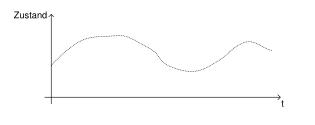
\includegraphics [scale=0.6]{images/kontinuierliche-modelle.jpg}
			\end{center}
		\subsubsection{Diskrete Modelle - schrittweise}
			\begin{description}
				\item[Beschreibung:] Endlich viele Zustandsübergänge pro Zeitintervall, Konstante Intervallänge (Alle Modellteile im Gleichtakt), Zustand bleibt bis zum nächsten Takt konstant, Beispiel: Wir füllen Badewanne in regelmäßigen Abständen mit Wassereimern
				\item[Zeit:]$\mathds{N}$
				\item[Zustandsraum:] beliebig
				\item[Input/Output:] beliebig
			\end{description}
			\begin{center}
				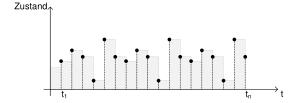
\includegraphics [scale=0.6]{images/diskret-schrittweise.jpg}
			\end{center}
		\subsubsection{Diskrete Modelle - Ereignisse}
			\begin{description}
				\item[Beschreibung:] Endlich viele Zustandsübergänge pro Zeitintervall, Modelle entwicklen sich durch Ereignisse, Zustand bleibt bis zum nächsten Ereigniss konstant, Beispiel: Wir füllen Badewanne mit Wassereimern immer dann, wenn wir angerufen werden
				\item[Zeit:] $\mathds{R}$
				\item[Zustandsraum:] beliebig
				\item[Input/Output:] beliebig
			\end{description}
			\begin{center}
				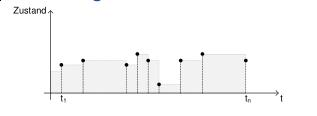
\includegraphics [scale=0.6]{images/diskret-ereignisse.jpg}
			\end{center}
		\subsubsection{Hybride Modelle}
			\begin{description}
				\item[Beschreibung:] Kombination aus kontinuierlichen und diskreten Modellen, es gibt sowohl Ereignisse welche durch die Zeit oder durch das Eintreten bestimmter Sitationen. Beispiel: Wir lassen Badewanne normal vollaufen und kippen alle 5 Minuten einen Wassereimer hinzu und immer dann wenn wir angerufen werden.
			\end{description}
			\begin{center}
				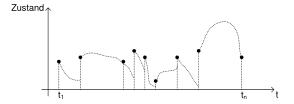
\includegraphics [scale=0.6]{images/hybrid.jpg}
			\end{center}
	\subsection{VVA von Modellen}
		\begin{description}
			\item[Verifikation:] Korrekte Transformation oder Beweisen
			\item[Validierung:] Korrektes Modell oder Testen
			\item[Akkreditierung:] Dritte Partei die das Modell (VV) bestätigt
		\end{description}
\section{Zelluläre Automaten}
	\subsection{Endliche Automaten}
		Die Formale Definition: $M=(Q,\Sigma,\Delta,\beta,q_{0},\Lambda)$ mit:
		\begin{itemize}
			\item Q endliche Menge an Zuständen
			\item $\Sigma$ endlichen Eingabealphabet
			\item $\Delta$ Ausgabealphabet
			\item $\beta$ Zustandübergangsfunktion: $\beta: Q \times \Sigma \rightarrow Q, \beta(p,a) = q$, mit $p,q \in Q, a\in \Sigma$
			\item $q_{0}$ Startzustand
			\item $\Lambda$ Ausgabefunktion
		\end{itemize}
		\begin{description}
			\item[Mealy-Automaten:] Ausgabe ist nur von der Eingabe abhängig. 
				\begin{itemize}
					\item $\Lambda: Q \times \Sigma \rightarrow \Delta$
					\item $\Lambda(p,a) = b$ mit $p\in Q, a \in \Sigma$, $ b\in \Delta$
				\end{itemize}
			\item[Moore-Automaten:] Ausgabe ist nur von dem Zustand abhängig.
				\begin{itemize}
					\item $\Lambda: Q \rightarrow \Delta$
					\item $\Lambda(p) = b$ mit $p\in Q$, $b\in \Delta$					
				\end{itemize}
		\end{description}
	\subsection{Defintion: zelluärer Automat}
		Die Idee von zellulären Automaten besteht darin mehere Automaten zu koppeln. Die Art der Koppelung bezeichnet man auch als Nachbarschaft. Anstelle von expliziten Eingaben, ändert sich der Zustand eines Automaten in Abhängigkeit von dessen Nachbarn. Nachfolgend ist die formale Definition eines zellulären Automaten: $CA=(L,N,S,G,G_{init},R)$ definiert durch:
		\begin{itemize}
			\item $L$ dem Zellraum, $L \subset \mathds{R}^{d}$ wobei d: d-dimensionaler Raum, somit ist L die Menge der homogen (gleichmaßig) über dem Raum verteilter Zellen. Jede Zelle wird durch ihre Position $r\in L$ bezeichnet.
			\item $N(r) := \{r+c_{i}:c_{i} \in \mathbf{N}_{diff(b)}, i = 1,\dots,b\}$ mit $\mathbf{N}_{diff(b)}$ der Offset, der die Nachbarn bestimmt, b ist die Anzahl der nächsten Nachbarn im Raum (2 für dimensional, 3 für Dreiecke usw \dots).
			\item $S$ der endliche Zustandsraum  mit $\forall r \in L : s(r) \in S (s : L \rightarrow S)$
			\item G der Zustand des zellulären Automaten, $G \in S^{|L|}$,$G := (s(r_{1}),\dots,s(r_{|L|})) = (s(r_{_{i}})_{r_{_{i}}} \in L)$
			\item $G_{init}$ der initiale Zustand des zellulären Automaten, $G_{init} \in S^{|L|}$
			\item $R$ die Zustandsüberführungsfunktion
		\end{itemize}
		Die Definition scheint jetzt sehr komplex. Wir werden diese jedoch später in einem Beispiel erläutern.Die Wahl der Nachbarschaft ist frei wählbar, es gibt jedoch zwei typische Nachbarschaften.\\
		\begin{enumerate}
		\item von-Neumann-Nachbarschaft: Nachbarn welche mit einer \glqq langen\grqq\ Seite an die Zelle.
		\item Moore-Nachbarschaft: alle benachbarten Zellen (alle Zellen welche eine Zelle berühren)
		\end{enumerate}
		Die Ränder des Automaten können verschieden behandelt werden. Entweder der Automat endet d.h. die Anzahl der Nachbarn an der Randzellen ist kleiner und die gedachten außerhalb liegenden Zellen haben einen festen Zustand oder die Welt ist ein Torus d.h. der Nachbar der Zelle am Rand ist auf der gegenüberliegenden Seite.\\
		Bisher wurde nicht geklärt wie wir die Schritte des Automaten berechnen. Mögliche Strategien wären:
		\begin{itemize}
			\item pro Schritt wird nur eine Zelle berechnet, Problem: Reihenfolge der Zellen
			\item alle Zellen pro Schritt berechnet und diese arbeiten auf den aktuellen Zustand der Nachbarn
			\item alle Zellen pro Schritt aber mit dem Zustand der Nachbarn aus dem vorigen Schritt
		\end{itemize}
	\subsubsection{Beispiel}
		Nachfolgend einige Beispiele für zelluläre Automaten.\\
		Beispiel 1: 1-dimensionale zelluläre Automaten\\
		$CA = (L,N,S,G,R)$ mit:
		\begin{itemize}
			\item $L \subseteq \mathds{Z}$(der Zellraum ist ein Band)
			\item $N_{diff(b)} = \{1,-1\}$(der linke und der rechte Nachbar)
			\item $S =$\{dead,alive\}(Zellen sind tot oder lebendig)
			\item  $G_{init} = \{s(r_{1},\dots,s(r_{ |l|}))\}\setminus \frac{|L|}{2}:s(r_{i})=$dead und $s(r_{\frac{|L|}{2}})=$ alive (alle Zellen sind tot ausser die Zelle mit dem Index $\frac{|L|}{2}$ sind tot)
			\item $R=$ die verwendete Regel.
		\end{itemize}
		Nachfolgend wird das Prinzip der Regel eingeführt. Nehmen wir an wir wählen eine Zelle auf dem Band mit dem Index $i$. Der Zustand dieser Zelle kann nach der obigen Definition nur von den beiden Nachbarzellen abhängen, da  $N(r) := \{r+c_{i}:c_{i} \in \mathbf{N}_{diff(b)}, i = 1,2\}$ mit $N_{diff(b)} = \{1,-1\}$ folgt $N(i)=\{i-1,i+1\}$, und von sich den eignen Zustand. Somit interessieren uns alle verschiedenen Anordnungen von $i-1,i,i+1$ mit den Belegungen $S={0,1}$ (0 nachfolgend für dead, 1 nachfolgend für alive). So ergeben sich 8 verschiedene Anordnungen. Für jede Anordnung müssen wir angeben wie sich die mittlere Zelle i entwickelt. Dieses geschieht über die Angabe der Regel in Binärcodierung. Nachfolgend ein Beispiel für Regel 42. \\
		Als erstes stellen wir $[42]_{10}$ als binär da. $42= 0*2^{7}+0*2^{6}+1*2^{5}+0*2^{4}+1*2^{3}+0*2^{2}+1*2^{1}+0*2^{0}=0*128+0*64+1*32+0*16+1*8+0*4+1*2+0*1=[00101010]_{2}$ und tragen das Ergebnis in die Tabelle ein.
		\begin{center}
			\begin{tabular}{|c|c|c|c|c|c|c|c|c|}
			\hline Muster & 111 & 110 & 101 & 100 & 011 & 010 & 001 & 000 \\ 
			\hline Neuer Zustand von i & 0 & 0 & 1 & 0 & 1 & 0 & 1 & 0    \\ 
			\hline 
			\end{tabular} 
		\end{center}
		Nachfolgend die Entwicklung des Automaten mit der Länge 5 über 2 Generationen mit der Annahme das die Zellen außerhalb des Randes den Wert 0 haben. In der Startkonfiguration haben alle Zellen haben den Wert 1.
		\begin{center}
			\begin{tabular}{|c||c|c|c|c|c||c|}
			\hline 0 & 1 & 1 & 1 & 1 & 1 & 0 \\ 
			\hline 0 & 1 & 0 &  0& 0 & 0 & 0 \\ 
			\hline 0 & 0 & 0 & 0 & 0 & 0 & 0 \\ 
			\hline 
			\end{tabular} 
		\end{center}
		Für mehre Dimensionen funktioniert dies Analog. Siehe Vorlesungsfolien.
		\newpage
\section{Discrete Event System Specification (DEVS)}
	\subsection{Vergleich zu zellulären Automaten}
		Im Vergleich zu zellulären Automaten ist in DEVS die Positionierung der einzelnen Bausteine egal und die Kommunikation kann mit belieben Komponenten erfolgen, nicht wie bei den CA mit den unmittelbar anliegenden Nachbarn. Mit DEVS ist es möglich ein System sowohl durch Dekomposition einzelne Bausteine zu verfeinern als auch durch Komposition die Bausteine wieder zusammen zu fassen. Dadurch ist es möglich in DEVS ein System beliebig fein/grob zu spezifizieren. Der Formalismus ist diskret Ereignisorientiert d.h. wir springen von Ereignis zu Ereignis.
	\subsection{DEVS: Atomare Modelle}
		Ein atomares Modell besitzt einen Zustand in diesem das System über einen definierten Zeitraum (auch unendlich lange) verweilt. Der Zustand ändert sich erst wenn ein Ereignis eintritt oder die Verweilzeit abgelaufen ist. Zu dem Ereignis gehört die aktuelle Zeit. Die Kombination von Zustand, Ereignis und der aktuellen Zeit entscheidet in welchem neuen Zustand das System übergeht. Die Zustandsüberführung kann durch ein externes Ereignis(direkte Eingabe) oder ein internes Ereignis(Verweilzeit) ausgelöst werden. Ausgehend durch diese Betrachtung ergibt sich folgende formale Spezifikation: $DEVS = (X,Y,S,\beta_{int},\beta{ext},ta,\lambda)$ mit: 
		\begin{itemize}
			\item $X$ die Eingabemenge
			\item $Y$ die Ausgabemenge
			\item $S$ die Menge der Zustände
			\item $ta: S \rightarrow \mathds{R}^{+}_{0,\infty}$ Zeitfortschrittfunktion weist jedem Zustand eine Zeitspanne zu, in die dieser Zustand von sich aus bestehen bleibt bevor ein interner Zustandsübergang ausgelöst wird
			\item $\beta_{int}: S \rightarrow S$ interne Übergangsfunktion (zeitgetriggerte Ereignisse)
			\item $\beta_{ext}: Q \times X \rightarrow S$ externe Übergangsfunktion (situative Ereignisse) mit $Q=\{(s,e)|s\in S, 0 \leq e \leq ta(s)\}$
			\item $\lambda: S \rightarrow Y$ Ausgabefunktion
		\end{itemize}
		Nachfolgend zu den Zustandsänderungen ist folgendes zu sagen: bei internen Ereignissen möchte das Modell eine Zustandsüberführung zu einem bestimmten Zeitput ($ta(s) \rightarrow tonie$) durchführen (tonie = time of next event), bei externen Ereignissen bekommt das Modelle eine Nachricht und ändert aufgrund der Eingabe seinen Zustand.\\
		Die Atomaren Modelle werden wir später nutzen um einzelne Komponenten in den gekoppelten Modellen zu spezifizieren.
	\subsection{DEVS: Gekoppelte Modelle}
		Ein gekoppeltes Modell ist eine Dekompostion eines Atomaren Modell. Nachfolgend die formale Definiton: $DEVS = (X,Y,D,\{M_{d}|d \in D\}.EIC,EOC,IC,Select)$ mit:
		\begin{itemize}
			\item $X$ die Eingabemenge
			\item $Y$ die Ausgabemenge
			\item $D$ Menge mit Namen von den Komponenten
			\item $\{M_{d}|d \in D\}$ eine Menge von DEVS-Modellen wobei jedes Modell ein Name $\in D$ besitzt
			\item $EIC$ Menge der externen Eingabekoppelungen (Eingabeports)
			\item $EOC$ Menge der externen Ausgabekoppelungen (Augabeports)
			\item $IC$ Menge der internen Koppelungen (interne Verbindung von Komponenten)
			\item $Select: 2^{D} \rightarrow D$ die Funktion, die bestimmt wenn mehrere Komponenten ein internes Ereignis ausführen wollen, welche Komponente priorisiert wird
		\end{itemize}
	\subsection{Darstellung}
		Eine übliche Darstellungsform sind geschachtelte Rechtecke. Die Koppelungen werden dabei durch gerichtete Pfeile von und zu Dreiecken die auf den Rändern der Rechtecke positioniert sind und nach außen zeigen wenn sie Ausgabeports und nach innen zeigen wenn sie Eingabeports repräsentieren.
		\begin{center}
			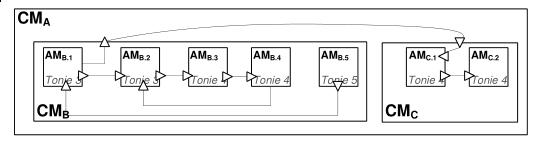
\includegraphics[scale=0.6]{images/devs-boxes.jpg}
		\end{center}
		Eine weitere Möglichkeit ist die Darstellung in Form eines hierarchisch aufgebauten Modellbaum. Dabei sind jedoch nicht alle nötigen Informationen bekannt die für die Berechnungen auf dem Modell notwendig sind.
		\begin{center}
			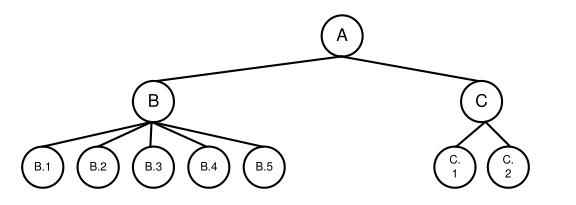
\includegraphics[scale=0.5]{images/devs-baum.jpg}
		\end{center}
		Für die Darstellung eine Ausführungssemantik entsprechende sind noch die Begriffe Koordinatoren und Simulatoren zu klären. In einen Prozessorbaum sind alle gekoppelten Modelle Koordinatoren und alle atomare Modelle Simulatoren. Zusätzlich wird ein Root-Koordinator eingeführt welcher die Wurzel des Prozessorbaumes bildet. Diese Unterteilung ist nötig für die Ausführsemantik, welche wir nachträglich noch erläutern werden.
	\begin{center}
			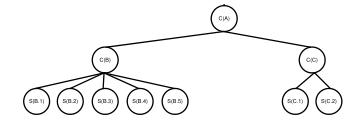
\includegraphics[scale=0.5]{images/devs-prozessorbaum.jpg}
	\end{center}
	\subsection{PDEVS: Atomare Modelle}
	PDEVS basiert auf DEVS und kommt ohne die select Funktion aus was die parallele Ausführung von internen Ereignissen erlaubt. Die PDEVS-Modelle sind analog zu den DEVS-Modellen aufgebaut, bestehen also aus gekoppelten Modellen und atomaren Modellen. Die atomaren Modelle in PDEVS sind wie folgt definiert: $M=(X,Y,S,\delta_{int},\delta_{ext},\delta_{con},\lambda,ta)$ mit:
	\begin{itemize}
		\item $X = \{(p,v)|p \in inPorts \wedge v \in X_{p}\}$, eine Menge aus Tupeln (Eingabeport,Eingabewert), v ist aus der Menge der möglichen EIngabewerte in p: $X_{p}$
		\item $Y = \{(p,v)|p \in outPorts \wedge v \in >_{p}\}$, eine Menge aus Tupeln (Ausgabeport,Ausgabewert), v ist aus der Menge der möglichen Ausgabewerte in p: $Y_{p}$
		\item $S$ die Menge der Zustände
		\item $\delta_{int}: S \rightarrow S$ die interne Übergangsfunktion
		\item $\delta_{ext}: Q \times X^{b}  \rightarrow S$ die externe Übergangsfunktion, $Q=\{(s,e)|s \in S \wedge 0 \leq e \le ta(s)\}$ die Menge aus Tupeln von Zuständen und der Zeit ($e = $ elapsedtime) in dem jeweiligen Zustand, $X^{b}$ bezeichnet eine Multimenge aus Elementen in X
		\item $\delta_{con}: S \times X^{b} \rightarrow S$ die konfluente Übergangsfunktion
		\item $\lambda: S \rightarrow Y^{b}$ die Ausgabefunktion
		\item $ta: S \rightarrow \mathds{R}^{+}_{0,\infty}$ die Zeitfortschrittsfunktion
	\end{itemize}
	\subsection{PDEVS: Gekoppelte Modelle}
	Die gekoppelten Modelle sind wie folgt definiert: $C = (X,Y,D,\{M_{d}|d \in D\}, EIC,EOC,IC)$ mit:
	\begin{itemize}
		\item $X = \{(p,v)|p \in inPorts \wedge v \in X_{p} \}$
		\item $Y = \{(p,v)|p \in outPorts \wedge v \in Y_{p} \}$
		\item $D$ die Menge der Namen der Komponenten
		\item $\forall d \in D$ gilt: $M_{d} =(X_{d},Y_{d},S,\delta_{int},\delta_{ext},\delta_{con},\lambda,ta)$ ist ein PDEVS-Modell mit $X_{d} = \{(p,v)|p \in inPorts \wedge v \in X_{p}\}$ und $Y_{d} = \{(p,v)|p \in outPorts \wedge v \in Y_{p}\}$
		\item $EIC \subseteq \{((C,ip_{c},(d,ip_{d}))|ip_{c} \in inputPorts) \wedge d \in D \wedge ip_{d}  \in inPorts_{d} \}$ die Menge der externen Eingabekoppelungen, die die EIngabeports des gekoppelten Modells mit den Eingängen der Komponenten verbindet
		\item $EOC \subseteq \{((d,op_{d},(C,op_{d}))|pc_{c} \in outPorts) \wedge d \in D \wedge op_{d}  \in outPorts_{d} \}$ die Menge der externen Ausgabekoppelungen, die die Ausgänge der Komponenten mit den Ausgabeports des gekoppelten Modells verbinden
		\item $IC \subseteq \{((a,op_{a},(b,ip_{b}))|a,b \in D \wedge op_{a}  \in outPorts_{a} \wedge ip_{b} \in inPorts_{b} \}$ die Menge der internen Koppelungen, die Ausgabeports der Komponenten mit den Eingabeports anderer Komponenten verbindet
	\end{itemize}
	Nach den ganzen Definitionen erläutern wir nun die Ausführsemantik.
	\subsection{Ausführsemantik}
	Nachfolgend gehen wir davon aus, dass das PDEVS Modell aus einem gekoppelten Modell besteht, über welchem nur der Rootcoordinator eingetragen ist.
	\begin{center}
		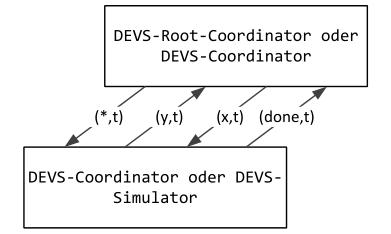
\includegraphics[scale=0.5]{images/devs-protokoll.jpg}
	\end{center}
	\begin{description}
	 	\item[Root-Koordinator:] Solange die Simulation nicht beendet ist, führt der Root-Koorinator folgende Schritte aus.
	 		\begin{enumerate}
		 		\item Senden von $(*,t)$ zum Kind (ist der Koordinator für das gekoppelte Modell)
		 		\item Warten auf eine Ausgabe y von dem Kind
		 		\item Senden einer Eingabe x zum Kind
		 		\item Warten auf $done(t)$ Nachricht von Kind
	 		\end{enumerate}
	 	\item[Koordinator:] Koordinatoren aktivieren die Kinder und leiten die eingehende Nachrichten an Kinder bzw. an höhere Koordinatoren weiter. Je nach Art der Nachricht reagiert der Koordinator anderes.
	 		\begin{enumerate}
	 			\item $(*,t)$ Nachricht empfangen
	 				\begin{enumerate}
		 				\item Senden von $(*,t)$ an alle imminenten Kinder (Kinder dessen tonie =t)
		 				\item Warten auf Ausgabe y von den imminenten Kindern
		 				\item Senden von Ausgabe y zum höheren Koordinator
		 				\item Warten auf $(x,t)$ Nachricht vom Vater
	 				\end{enumerate}
	 			\item Senden von $(x,t)$ Nachrichten an alle Kinder
	 			\item Warten von $done(t)$ Nachrichten von allen Kindern
	 			\item Aktualisierung von tonie auf das Minimum von allen Kindern
	 			\item Senden von $done(tonie)$ zum Vater
	 		\end{enumerate}
	 	\item[Simulator:] Simulatoren machen die eigentlichen Zustandsveränderungen
	 		\begin{enumerate}
		 		\item Wenn $(*,t)$ empfangen
		 			\begin{enumerate}
			 			\item Die Ausgabe $\lambda(S)$ berechnen
			 			\item Ausgabe an Vater senden
			 			\item Warten auf $(x,t)$ Nachricht 
			 			\item Wenn x Nachricht leer ist (Keine Eingabe von Aussen): Interner Übergang $\delta_{int}(S)$
			 			\item Sonst: Konfluenter Übergang (Eingabe von Aussen $\delta_{con}$ 
		 			\end{enumerate}
		 		\item Wenn $(x,t)$ empfangen
		 			\begin{enumerate}
			 			\item Berechnen der vergangenen Zeit $e = t - t_{last}$ (Empfangene Zeit - Zeit des letzten Event des Knotens)
			 			\item Externer Übergang $\delta_{ext}(S,e,x)$
		 			\end{enumerate}
		 		\item Aktualisieren der Zeit des letzten Events $t_{last} = t$
		 		\item Aktualisieren der Zeit des nächsten Events $tonie = t$
		 		\item Senden von $done(tonie)$ zum Vater
	 		\end{enumerate}
	\end{description}
	\subsection{Vergleich von DEVS und PDEVS}
	PDEVS ermöglicht es uns parallele Ereignisse (interne und externe Ereignisse gleichzeitig) einfacher zu beschreiben. In PDEVS gibt es keine Select-Funktion welche die Prioritäten der Komponeten angibt. Mehre Komponenten können gleichzeitig einen intern Zustandsübergang ausführen. Kollisionen von internen und externen Ereignissen wird auf atomarer Ebene aufgelöst durch $\delta_{conf}$. Der Spezialfall, dass beide Generatoren zu gleichen Zeit eine Ausgabe erzeugen können, führt zur Erweiterung $X^{b}$

\section{Petrinetze}
	Die Modellierung mittels Petrinetzen geht zurück auf Adam Petri. Der Formalismus Petrinetz ist ein schlanker, visueller Modellierungsformalismus, mit denen nebenläufige Prozesse mit diskreten Elementen simuliert werden können. Die Zentrale Idee hierbei ist, dass die Interaktion von Prozessen durch das Verbrauchen und Generieren von Ressourcen nachempfunden wird. Die Bestandteile  sind:
	\begin{itemize}
		\item Stellen
		\item Marken
		\item Transitionen
	\end{itemize}
	\subsection{Diskrete Systeme}
	Petrinetze beschreiben diskrete Systeme, deren Änderung sich in diskreten Schritten vollzieht. Es sind eher generelle Eigenschaften des Systems von Interesse - die Verifikation ist wichtiger als die Simulation.
	\begin{description}
		\item[Sicherheit - Es soll nichts Verbotenes passieren können (bad things never happen)] Anforderungen an die Stellen bzw. Markierungen, z.T. obere und untere Schranken, die die Markierung einer Stelle nicht unter- oder überschreiten darf.
		\item[Lebendigkeit - Das System soll nicht steckenbleiben (good things eventually happen)] Anforderungen an die Transitionen bzw. an das Schaltverhalten und fordern z.B. dass das Hintereinanderschalten bestimmter Transitionen die Markierung bewahrt.
	\end{description}
	\subsection{Definition: Netz und Stellen-Transitions-System}
		Nachfolgend die formale Definition eines Netzes: 
		\begin{description}
			\item[Stellen:] Sind Plätze auf denen Marken liegen können ($S$)
			\item[Transitionen:] Sind Verbindungen zwischen Stellen welche Marken konsumieren und produzieren können ($T$)
			\item[Flussrelationen:] Beschreiben die Verbindungen zwischen Stellen und Transitionen ($F$)
			\item[Netz:] $N=(S,T,F)$, mit $S \cap T = \emptyset$ (die Namen von den Stellen und den Transitionen überschneiden sich nicht), $F \subseteq (S \times T) \cup (T \times S)$ (die Kanten verlaufen zwischen Stellen zu Transitionen und Transitionen zu Stellen)
		\end{description}
		Ausgehend von dieser Beschreibung definieren wir ein Stellen-Transitions-System $Y=(S,T,F,K,W,M_{0})$ mit:
		\begin{itemize}
			\item $(S,T,F)$ ist ein Netz
			\item $K: S \rightarrow \mathbf{N} \cup \{\infty\}$. weist jeder Stelle eine maximale Kapazität zu
			\item $W: F \rightarrow \mathbf{N}$, weist jeder Kante ein Gewicht zu
			\item $M_{0}: S \rightarrow \mathbf{N}_{0}$, weist jeder Stelle einen Anzahl an Ausgangsmarken zu wobei $\forall s \in S : M_{0} \leq K(s)$ (die Anzahl muss unter der definierten Kapazität liegen)
		\end{itemize}
		Bis jetzt können wir ein statisches Netz definieren, d.h. wir haben noch eine Aktion. Dies werden wir mit den nachfolgenden Definitionen beheben.
		\begin{description}
			\item[Vorbereich einer Transtion:] $\bullet x = \{y|(y,x)\in F, y \in S, x \in T\}$, alle Stellen welche  mit einer Transition verbunden sind
			\item[Nachbereich einer Transtion:] $x\bullet = \{y|(x,y)\in F, y \in S, x \in T\}$, alle Stellen welche von einer Transition verbunden sind
			\item[Aktiviertheit einer Transtion:]
				\begin{itemize}
					\item $\forall s \in \bullet t \cap t \bullet . M(s) \leq K(s) - W(t,s) + W(s,t)$
				\end{itemize}
		\end{description}

\section{Prozessalgebren}
	\subsection{Rückblick}
		Alle bisherigen Formalismen haben eines gemeinsam: eine statische Kommunikation- und Kompositionsstruktur. So sind bei Zellulären Automaten die Nachbarschaften fest definiert und ändern sich nicht, bei DEVS ändern sich die Koppelungen und die Komponenten nicht und bei Petrinetzen ändert sich nicht die Anzahl an Knoten und Kanten. Nachfolgend werden wir einen Formalismus kennen lernen der besonders geeignet ist Interaktionen/Kommunikation zu modellieren.
	\subsection{$\pi$-Kalkül}
		Im $\pi$-Kalkül wird das System durch interagierende Prozesse beschrieben. Die Kommunikation der Prozesse geschieht über Kanäle, welche durch Namen definiert sind. Der Kommunikationsinhalt sind immer die Namen von den Kanälen. Nachfolgend wird die Syntax des Kalküls beschrieben.
		\begin{itemize}
			\item $P::= 0$ P ist der 0-Prozess (ist terminiert)
			\item $P||Q$ P und Q laufen parallel
			\item $c!(v).P$ Prozess wartet bis v auf Kanal c gesendet werden kann und verhält sich dann wie P
			\item $c?(x).P$ Prozess wartet auf Eingabe auf Kanal c und bindet die Eingabe an die Variable x und verhält sich dann wie P
			\item $(\nu x).P$ Erstelle Kanal x und fortsetzen wie Prozess P
			\item $!P$ Prozess findet unendlich oft nebenläufig statt
			\item $P+Q$ Prozess verhält sich wie P xor Q
		\end{itemize}
		Wir wissen nun wie man Prozesse/Systeme beschreibt jedoch können wir keine Reduktionen durchführen d.h. wir können noch keine Prozesse laufen lassen. Deshalb werden folgende Reduktionsregeln eingeführt. Im Zähler steht dabei die Vorbedingung, im Nenner steht dabei die Entwicklung des Prozesses.
		\begin{description}
			\item [Nebenläufigkeit $P||Q$:] $\frac{P \rightarrow P'}{P||Q \rightarrow P'||Q}$ d.h. wenn sich der Prozess P zu P' entwickelt ändert sich in der parallel Ausführung der Prozess Q nicht.
			\item [Kommunikation $c!(v).P || c?(x).Q$:] $\frac{P \rightarrow P'}{P || Q\{v/x\}}$ d.h. $c?(x).Q$ hört auf Kanal c auf ein x, $c!(v).P$ sendet auf Kanal c ein v, so wird in Q alle x durch v ersetzt.
		\end{description}






\end{document}